%%%%%%%%%%%%%%%%%%%%%%%%%%%%%%%%%%%%%%%%%%%%%%%%%%%%%%%%%%%%%%%%%%%%%%%%%%%%%%%%%%
\begin{frame}[fragile]\frametitle{}
\begin{center}
{\Large Overview of Methods}

{\tiny (Ref: Reinforcement Learning Series: Overview of Methods - Steve Brunton )}
\end{center}
\end{frame}





%%%%%%%%%%%%%%%%%%%%%%%%%%%%%%%%%%%%%%%%%%%%%%%%%%%%%%%%%%%%%%%%%%%%%%%%%%%%%%%%%%
\begin{frame}[fragile]\frametitle{Components}

\begin{center}
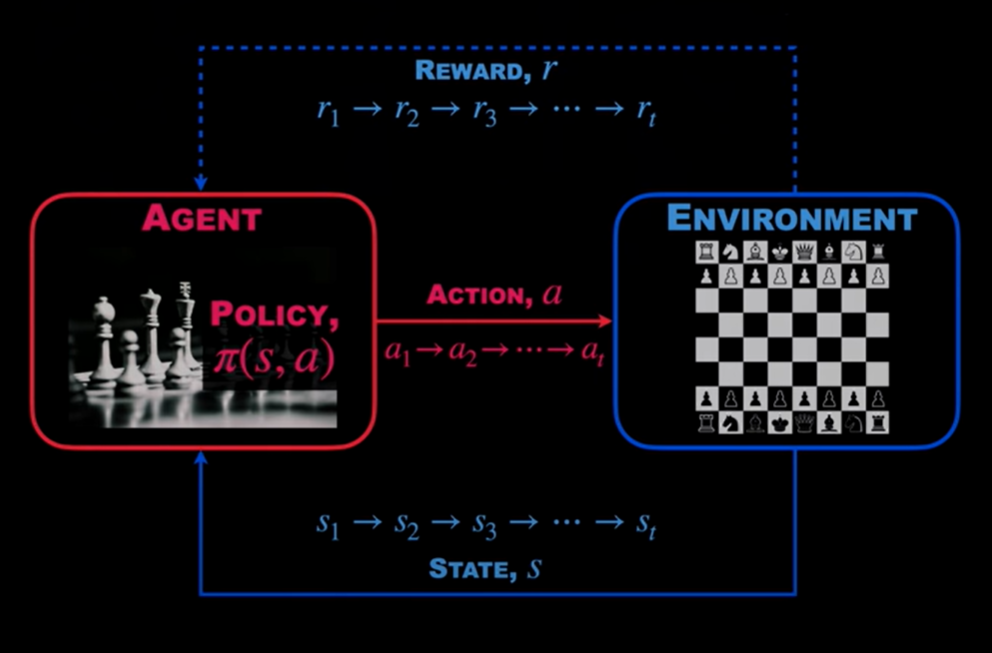
\includegraphics[width=\linewidth,keepaspectratio]{rl157}
\end{center}

\end{frame}

%%%%%%%%%%%%%%%%%%%%%%%%%%%%%%%%%%%%%%%%%%%%%%%%%%%%%%%%%%%%%%%%%%%%%%%%%%%%%%%%%%
\begin{frame}[fragile]\frametitle{Explanation: Components}

\begin{itemize}
\item Agent interacts with the world (Environment) through a set of actions ($a$). 
\item Actions can be discrete (chess) or continuous (moving robot).
\item Environment gives information about its State ($s$) using which Agent decides the Action.
\item Environment also gives information about the Reward ($r$) after the Action is carried, which is based on achieve-ability or closeness to the final goal.
\item Agent uses Policy ($\pi$) which is a probability of action $a$ given state $s$ ie $\pi (s,a) = Pr(a = a| s = s)$. Probability can be deterministic or probabilistic. Basically some kind of set of rules to decide the next action, to maximize rewards.
\item For a particular policy, one can associate an expected 'Value' to each State for bringing sum of all future rewards. $V_{\pi}(s) = E (\sum {\gamma}^t r_t | S_0 = s)$ where $\gamma$ is discount rate.
\item The State space is enormously large, say for Chess, number of chess board configurations is huge.
\item Goal of Reinforcement Learning is to optimize Policy (or find best policy) to maximize future Rewards. Very hard problem, RnD going on for 100+ years. We can use Machine Learning at some places.
\end{itemize}

\end{frame}



%%%%%%%%%%%%%%%%%%%%%%%%%%%%%%%%%%%%%%%%%%%%%%%%%%%%%%%%%%%%%%%%%%%%%%%%%%%%%%%%%%
\begin{frame}[fragile]\frametitle{Model Types}

\begin{center}
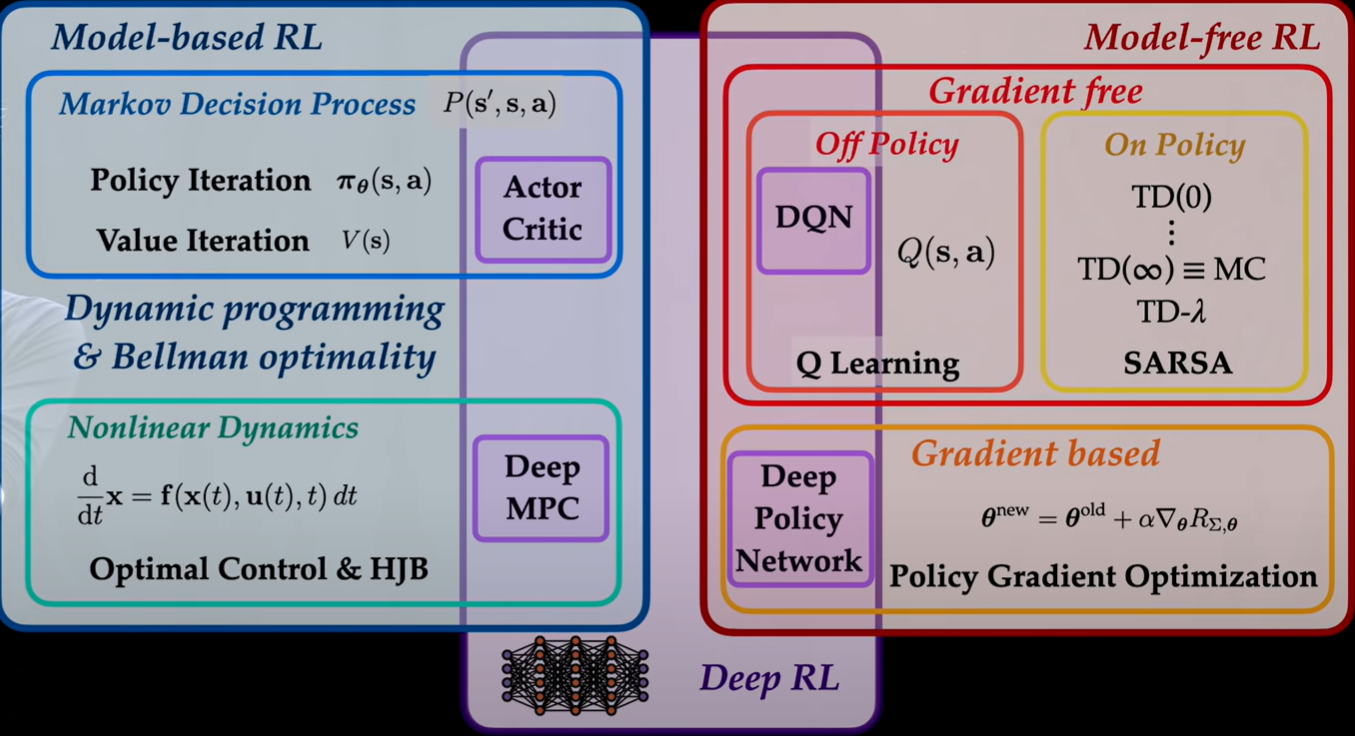
\includegraphics[width=\linewidth,keepaspectratio]{rl158}
\end{center}

\end{frame}

%%%%%%%%%%%%%%%%%%%%%%%%%%%%%%%%%%%%%%%%%%%%%%%%%%%%%%%%%%%%%%%%%%%%%%%%%%%%%%%%%%
\begin{frame}[fragile]\frametitle{Explanation: Model-based}

\begin{itemize}
\item First level organization of RL based approaches is: Model-based or Model-Free.
\item Model means some logic representing behavior of the Environment. Say, some processes are Markov based, some are Differential Equation based, etc. So, these are Model-based RLs.
\item In Markov Decision Processes, there is a known probability from going from state $s$ to state $s'$ given action $a$. No history is taken into account but just the current action decide the state. 
\item Here, Policy Iteration and Value Iteration approaches are used to find the optimal Policy. Simulation of all possibilities. 
\item Iterations are done using Dynamic Programming (why? intermediate states are saved and not computed all the time)
\item In practice these are all brute force searches, not scale-able for high dimensional systems.
\end{itemize}

\end{frame}

%%%%%%%%%%%%%%%%%%%%%%%%%%%%%%%%%%%%%%%%%%%%%%%%%%%%%%%%%%%%%%%%%%%%%%%%%%%%%%%%%%
\begin{frame}[fragile]\frametitle{Explanation: Model-free}

\begin{itemize}
\item In practice, you don't have model, ie. you don't have your Opponent's model in Chess, which will tell what moves s/he is going to do. Try Model-Free approaches: Gradient-free and Gradient-based.
\item Gradient-based: If you can parameterize the Policy by some $\theta$, then during optimization, taking gradient to find maxima/minima is possible.
\item Gradient-free: either `Off Policy' (may try some random things occasionally, e.g. Q-Learning) or `On Policy' (always try to play best game, most reward, e.g. SARSA). 
\item Q (Quality) Learning: can derive Policy and Value function. Can take sub-optimal paths, at times. Good for imitation learning (see someone play). 
\item All this approaches have sub-approaches leveraging Deep Learning. E.g. Q-Learning with Deep Learning is DQN (Deep Quality Network). THIS IS WHAT WE DO typically.
\end{itemize}

\end{frame}



